\documentclass[11pt,a4paper]{article}

\usepackage[T1]{fontenc}
\usepackage[utf8]{inputenc}
\usepackage{lmodern}
\usepackage[margin=2.4cm]{geometry}
\usepackage{microtype}
\usepackage{graphicx}
\usepackage{float}
\usepackage[export]{adjustbox}
\usepackage{booktabs}
\usepackage{longtable}
\usepackage{array}
\usepackage{enumitem}
\usepackage{xcolor}
\usepackage{caption}
\usepackage{subcaption}
\usepackage{fancyhdr}
\usepackage{titlesec}
\usepackage{tikz}
\usetikzlibrary{positioning,arrows.meta,shapes.geometric,fit,calc}
\usepackage[colorlinks=true,linkcolor=black,urlcolor=blue!50!black,citecolor=black]{hyperref}

\definecolor{brand}{HTML}{1D4ED8}
\definecolor{soft}{HTML}{EFF4FF}
\definecolor{rule}{HTML}{CBD5E1}

\setlength{\parindent}{0pt}
\setlength{\parskip}{0.55em}
\renewcommand{\arraystretch}{1.18}
\setlist{itemsep=0.15em,topsep=0.3em}
\captionsetup{font=small,labelfont=bf}

\titleformat{\section}{\Large\bfseries\color{brand}}{\thesection}{0.7em}{}
\titleformat{\subsection}{\large\bfseries}{\thesubsection}{0.6em}{}
\titlespacing*{\section}{0pt}{1.6em}{0.6em}
\titlespacing*{\subsection}{0pt}{1.1em}{0.4em}

\pagestyle{fancy}
\fancyhf{}
\fancyhead[L]{\small TaskBoard -- IT645 Project Report}
\fancyhead[R]{\small DA-IICT}
\fancyfoot[C]{\small\thepage}
\renewcommand{\headrulewidth}{0.3pt}

% Screenshot helpers. An image <name> is looked for as screens/<name>.<ext> and as ./<name>.<ext>
% (png, jpg, jpeg in lower or upper case). A labelled box is shown when it is missing.
\makeatletter
\newcommand{\findimg}[1]{%
  \gdef\imgfile{}%
  \@for\imgdir:=screens/,./\do{%
    \@for\imgext:=png,jpg,jpeg,PNG,JPG,JPEG\do{%
      \ifx\imgfile\@empty\IfFileExists{\imgdir#1.\imgext}{\xdef\imgfile{\imgdir#1.\imgext}}{}\fi}}}
\makeatother
\newcommand{\placeholder}[2]{\fbox{\parbox[c][4.5cm][c]{\dimexpr#2\linewidth-2\fboxsep-2\fboxrule\relax}{\centering\small Missing: \texttt{#1}}}}
\newcommand{\img}[2]{\findimg{#1}%
  \ifx\imgfile\empty\placeholder{#1}{#2}\else\includegraphics[width=#2\linewidth]{\imgfile}\fi}
% Top part only of a tall image: #1 name, #2 fraction of the height cut away at the bottom (0--1), #3 width as fraction of the line
\newcommand{\imgtop}[3]{\findimg{#1}%
  \ifx\imgfile\empty\placeholder{#1}{#3}\else\adjustbox{trim={0pt {#2\height} 0pt 0pt},clip,width=#3\linewidth}{\includegraphics{\imgfile}}\fi}
\newcommand{\shot}[3]{\begin{figure}[H]\centering\img{#1}{#2}\caption{#3}\end{figure}}
\newcommand{\shotpair}[5]{%
  \begin{figure}[H]\centering
  \begin{subfigure}[t]{0.485\linewidth}\centering\img{#1}{1}\caption{#2}\end{subfigure}\hfill
  \begin{subfigure}[t]{0.485\linewidth}\centering\img{#3}{1}\caption{#4}\end{subfigure}
  \caption{#5}\end{figure}}

\newcommand{\code}[1]{\texttt{#1}}

\begin{document}

% ------------------------------------------------------------ title page
\begin{titlepage}
\thispagestyle{empty}
\centering
{\large Dhirubhai Ambani University (DA-IICT), Gandhinagar\par}
\vspace{0.4em}
{\large Course IT645 -- Web and Mobile Development\par}
\vspace{3.2cm}
{\Huge\bfseries\color{brand} TaskBoard\par}
\vspace{0.6em}
{\Large A Kanban-based project and task tracker\par}
\vspace{0.3em}
{\large Project report\par}
\vspace{2.4cm}
\begin{tabular}{@{}ll@{}}
Faculty & Dr.\ Shruti Bhilare\\[0.3em]
Live application & \url{https://taskboard-gu4g.onrender.com}\\
Source code & \url{https://github.com/24Chessman/TaskBoard}\\
\end{tabular}

\vspace{1.8cm}
\begin{tabular}{@{}lll@{}}
\toprule
\textbf{Team member} & \textbf{Student ID} & \textbf{Modules}\\
\midrule
Naitik Sutariya & 202512006 & Tasks and Board, GitHub issue lookup\\
Harshal Prajapati & 202512013 & Authentication, Users, activity logger\\
Jay Trivedi & 202512123 & Projects and Teams\\
Jaydip & 202512090 & Comments, Activity feed, Dashboard\\
\bottomrule
\end{tabular}

\vfill
{\large November 2026\par}
\end{titlepage}

\tableofcontents
\clearpage

% ------------------------------------------------------------ 1
\section{Introduction}

\subsection{Purpose}
TaskBoard is a lightweight project and task tracker, a small version of tools such as Jira. Teams create projects, invite members and manage work on a Kanban board with four columns: To Do, In Progress, Review and Done. Every task carries a lead, a priority, labels and a due date. Members discuss a task in its comments, every change is written to an activity log, and a dashboard summarises progress.

The application is a full-stack MERN project (MongoDB, Express, React, Node.js) built for the course IT645. It is deployed as a single web service and is available at the address on the title page.

\subsection{Scope}
The system provides:
\begin{itemize}
  \item account registration, login and a profile page;
  \item projects with members and two project roles (owner and member), plus a global administrator;
  \item a board with drag-and-drop between columns by mouse, touch and keyboard;
  \item tasks with title, description, status, priority, lead, labels, due date and an optional link to a GitHub issue or pull request;
  \item comments on tasks, an append-only activity feed and a per-project dashboard;
  \item an administration page for users;
  \item a responsive interface that works from 360~px phone width upwards.
\end{itemize}
Out of scope are real-time updates, file attachments, notifications, several leads per task and ordering of cards inside a column.

% ------------------------------------------------------------ 2
\section{Requirements}

\subsection{Functional requirements by module}
\begin{longtable}{@{}p{3.1cm}p{12.4cm}@{}}
\toprule
\textbf{Module} & \textbf{Capabilities}\\
\midrule
\endhead
Authentication and users & Register, log in, current user; edit own name, email and password (current password required); search users; administrators change roles and delete users.\\
Projects and teams & Create, edit, archive and delete projects; add and remove members; the creator becomes owner; the last owner cannot be removed.\\
Tasks and board & Create, edit, delete tasks; change status; filter by lead, priority, label and search text; sort; drag and drop; GitHub issue link with title and open or closed state.\\
Comments & Add, edit and delete comments on a task.\\
Activity feed & Read-only history of project, member, task and comment events, newest first.\\
Dashboard & Task totals, tasks by status and priority, overdue and due-soon counts, tasks without a lead, workload per member, top labels, tasks created per day.\\
\bottomrule
\end{longtable}

\subsection{Roles and permissions}
There are two layers. The global role of a user is \code{user} or \code{admin}. Inside a project a member is \code{owner} or \code{member}. A global administrator counts as owner of every project.

\begin{table}[H]
\centering\small
\begin{tabular}{@{}p{7.2cm}p{8.2cm}@{}}
\toprule
\textbf{Action} & \textbf{Allowed for}\\
\midrule
Register, log in & anyone\\
Create a project & any logged-in user (becomes owner)\\
View a project, its tasks, comments, activity, dashboard & project members, administrator\\
Edit, archive, delete a project; manage members & project owner\\
Create a task; change a task status; add a comment & any project member\\
Edit a task & owner, the task creator, or the task lead\\
Delete a task & owner or the task creator\\
Edit a comment & its author only\\
Delete a comment & its author or the project owner\\
Change a user role; delete a user & administrator only\\
\bottomrule
\end{tabular}
\caption{Permission rules enforced by the server.}
\end{table}

\subsection{Non-functional requirements}
\begin{itemize}
  \item \textbf{Security:} hashed passwords, token-based authentication, server-side authorisation on every route, validated input.
  \item \textbf{Usability:} responsive layout from 360~px, keyboard access for the board and all menus, plain error messages.
  \item \textbf{Maintainability:} one folder per concern, files kept short, a written API contract and a design system document.
  \item \textbf{Deployability:} one build command and one start command; configuration only through environment variables.
\end{itemize}

% ------------------------------------------------------------ 3
\section{System architecture}

\subsection{Overview}
The browser loads a single-page React application. The application talks to a REST API built with Express. The API stores data in MongoDB Atlas through Mongoose and, for the issue lookup, calls the public GitHub API. In production one Node.js process serves both the API under \path{/api} and the built client files, so the application and the API share one origin and no cross-origin configuration is needed.

\begin{figure}[H]
\centering
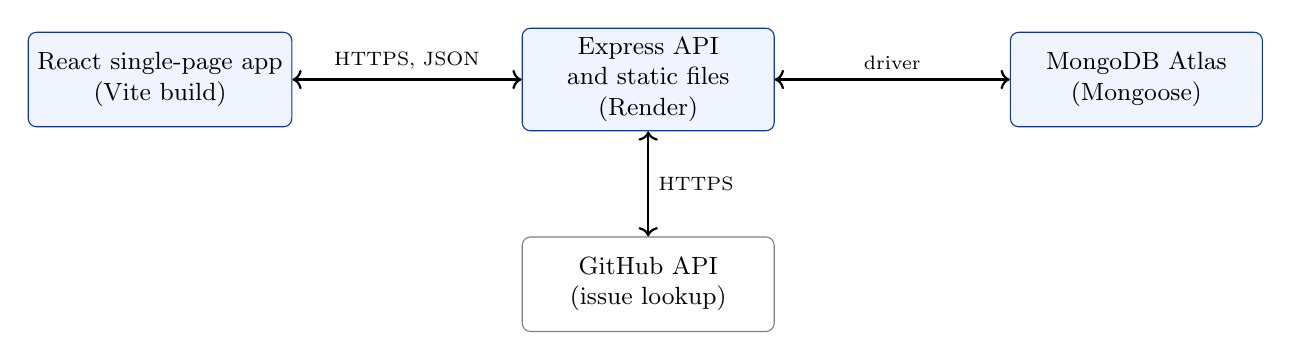
\begin{tikzpicture}[
  box/.style={draw=brand!70!black,fill=soft,rounded corners=3pt,minimum height=1.2cm,minimum width=3.2cm,align=center,font=\small},
  ext/.style={draw=black!50,fill=white,rounded corners=3pt,minimum height=1.2cm,minimum width=3.2cm,align=center,font=\small},
  arr/.style={-{Stealth[length=2.4mm]},thick}]
\node[box] (spa) at (0,0) {React single-page app\\(Vite build)};
\node[box] (api) at (6.2,0) {Express API\\and static files\\(Render)};
\node[box] (db) at (12.4,0) {MongoDB Atlas\\(Mongoose)};
\node[ext] (gh) at (6.2,-2.6) {GitHub API\\(issue lookup)};
\draw[arr,<->] (spa) -- node[above,font=\scriptsize]{HTTPS, JSON} (api);
\draw[arr,<->] (api) -- node[above,font=\scriptsize]{driver} (db);
\draw[arr,<->] (api) -- node[right,font=\scriptsize]{HTTPS} (gh);
\end{tikzpicture}
\caption{Runtime architecture.}
\end{figure}

\subsection{Technology stack}
Versions are the ones installed from the lock files when this report was prepared.
\begin{table}[H]
\centering\small
\begin{tabular}{@{}lll@{}}
\toprule
\textbf{Layer} & \textbf{Technology} & \textbf{Version}\\
\midrule
Runtime & Node.js & 18 or newer (22.19 used for testing)\\
Server & Express & 4.22.3\\
Server & Mongoose & 8.24.5\\
Server & jsonwebtoken, bcryptjs & 9.0.3, 3.0.3\\
Client & React, React Router & 18.3.1, 6.30.6\\
Client & Vite, Tailwind CSS & 8.3.5, 3.4.19\\
Client & axios, Recharts, lucide-react & 1.21.0, 3.10.1, 1.66.0\\
Client & @dnd-kit/core (drag and drop) & 6.3.1\\
Database & MongoDB Atlas & hosted\\
Hosting & Render web service & free tier\\
Quality & Postman collections, Newman 6.2.3, GitHub Actions & --\\
\bottomrule
\end{tabular}
\caption{Technology stack.}
\end{table}

\subsection{Server request pipeline}
Each request passes through the same chain in \code{app.js}: security headers, CORS policy, request logging, JSON body parsing, then the route. Routes add only the middleware they need: \code{auth} (valid token), \code{projectAccess} (membership), \code{requireProjectOwner}, \code{requireRole} and \code{activityLogger}. After the API routes, in production, a static handler serves the client; after that come the not-found handler and one central error handler that converts Mongoose validation errors, duplicate keys and bad identifiers into the standard error response.

\subsection{Repository layout}
\begin{itemize}
  \item \code{server/src}: \code{controllers} (8 files), \code{middleware} (9), \code{models} (5), \code{routes} (8), \code{config}, \code{scripts}, \code{utils}.
  \item \code{client/src}: \code{api}, \code{components} (grouped by feature), \code{context}, \code{hooks} (8), \code{pages} (14), \code{routes} (4 guards), \code{utils}.
  \item \code{docs}: product requirements, technical requirements, application flow, API contract, design system, eight Postman collections.
  \item \code{.github/workflows}: the continuous-integration workflow.
\end{itemize}

% ------------------------------------------------------------ 4
\section{Database design}
The database has five collections. Timestamps (\code{createdAt}, \code{updatedAt}) are kept on all of them.

\begin{figure}[H]
\centering
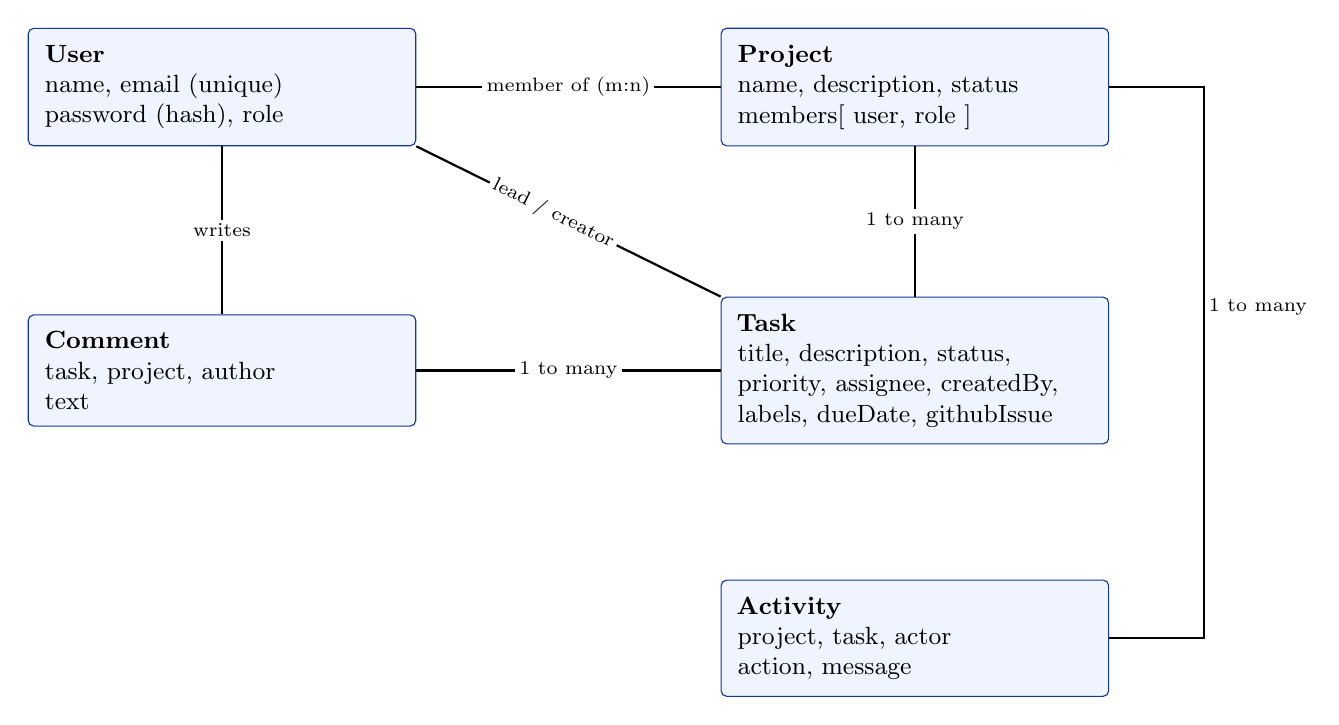
\begin{tikzpicture}[
  ent/.style={draw=brand!70!black,fill=soft,rounded corners=2pt,font=\small,align=left,inner sep=6pt,text width=4.5cm},
  rel/.style={thick},
  lab/.style={font=\scriptsize,fill=white,inner sep=1.5pt}]
\node[ent] (user) at (0,0) {\textbf{User}\\name, email (unique)\\password (hash), role};
\node[ent] (proj) at (8.8,0) {\textbf{Project}\\name, description, status\\members[ user, role ]};
\node[ent] (comm) at (0,-3.6) {\textbf{Comment}\\task, project, author\\text};
\node[ent] (task) at (8.8,-3.6) {\textbf{Task}\\title, description, status,\\priority, assignee, createdBy,\\labels, dueDate, githubIssue};
\node[ent] (act) at (8.8,-7.0) {\textbf{Activity}\\project, task, actor\\action, message};
\draw[rel] (user) -- node[lab]{member of (m:n)} (proj);
\draw[rel] (proj) -- node[lab]{1 to many} (task);
\draw[rel] (task) -- node[lab]{1 to many} (comm);
\draw[rel] (user) -- node[lab]{writes} (comm);
\draw[rel] (proj.east) -- ++(1.2,0) |- node[lab,pos=0.2,right]{1 to many} (act.east);
\draw[rel] (user.south east) -- node[lab,sloped,pos=0.45]{lead / creator} (task.north west);
\end{tikzpicture}
\caption{Entity relationships.}
\end{figure}

\subsection{Collections}
\begin{longtable}{@{}p{2.2cm}p{13.3cm}@{}}
\toprule
\textbf{Model} & \textbf{Fields and rules}\\
\midrule
\endhead
User & \code{name} (2--50 characters); \code{email} (required, unique, lower case, pattern-checked); \code{password} (minimum 6 characters, never returned by queries, hashed with bcrypt, 10 rounds); \code{role} (\code{user} or \code{admin}).\\
Project & \code{name} (3--80); \code{description} (up to 500); \code{status} (\code{active} or \code{archived}); \code{members}, an array of \code{\{user, role\}} where a user appears at most once and at least one member is an owner. Index on \code{members.user}.\\
Task & \code{project}; \code{title} (1--120); \code{description} (up to 2000); \code{status} (\code{todo}, \code{in\_progress}, \code{review}, \code{done}); \code{priority} (\code{low}, \code{medium}, \code{high}); \code{assignee} (optional, shown as ``Lead'' in the interface, must be a project member); \code{createdBy}; \code{labels} (at most 5, 1--20 characters each); \code{dueDate}; \code{githubIssue}, an embedded document with \code{url}, \code{title}, \code{state}. Indexes on project with status and project with due date.\\
Comment & \code{task}, \code{project}, \code{author}, \code{text} (1--1000). Index on task and creation time.\\
Activity & \code{project}, optional \code{task}, \code{actor}, \code{action} (nine values such as \code{task.created} or \code{comment.added}) and a readable \code{message} stored when the event is written. Append-only: no update or delete endpoint exists. Index on project and time.\\
\bottomrule
\end{longtable}

\subsection{Referential rules implemented in controllers}
MongoDB does not enforce foreign keys, so the controllers do:
\begin{itemize}
  \item Deleting a project deletes its tasks, comments and activity.
  \item Deleting a task deletes its comments.
  \item Deleting a user clears them as lead and removes them from projects, but keeps their comments and activity, which are then shown as ``Deleted user''. A user who is the only owner of a project cannot be deleted.
  \item Removing a member clears them as lead in that project.
\end{itemize}

% ------------------------------------------------------------ 5
\section{API design}
The API lives under \path{/api}, uses JSON, and has 29 endpoints plus a public health check. The full contract is in \code{docs/backend\_schema.md}.

\subsection{Conventions}
\begin{itemize}
  \item Success: \code{\{ success: true, data \}}; lists add \code{page}, \code{limit} and \code{total}.
  \item Error: \code{\{ success: false, message, errors: [\{ field, message \}] \}}.
  \item Status codes: 200, 201, 204 (delete, no body), 400 (validation, bad identifier), 401, 403, 404, 409 (duplicate), 429 and 502 (GitHub lookup).
  \item Paging: projects default 10 (maximum 50), tasks 50 (100), comments 50 (100), activity 10 (50).
  \item Task list filters: \code{status}, \code{priority}, \code{assignee}, \code{label}, \code{dueBefore}, \code{search}, \code{sort}, \code{page}, \code{limit}.
\end{itemize}

\subsection{Endpoints}
\begingroup\small
\begin{longtable}{@{}r l p{6.1cm} l p{3.0cm}@{}}
\toprule
\textbf{\#} & \textbf{Method} & \textbf{Path} & \textbf{Access} & \textbf{Purpose}\\
\midrule
\endhead
1 & POST & \path{/auth/register} & public & create account\\
2 & POST & \path{/auth/login} & public & log in\\
3 & GET & \path{/auth/me} & login & current user\\
4 & POST & \path{/projects} & login & create project\\
5 & GET & \path{/projects} & login & list projects\\
6 & GET & \path{/projects/:projectId} & member & one project\\
7 & PUT & \path{/projects/:projectId} & owner & update project\\
8 & PATCH & \path{/projects/:projectId/status} & owner & archive, reactivate\\
9 & DELETE & \path{/projects/:projectId} & owner & delete project\\
10 & POST & \path{/projects/:projectId/members} & owner & add member\\
11 & DELETE & \path{/projects/:projectId/members/:userId} & owner & remove member\\
12 & POST & \path{/projects/:projectId/tasks} & member & create task\\
13 & GET & \path{/projects/:projectId/tasks} & member & list tasks\\
14 & GET & \path{/projects/:projectId/tasks/:taskId} & member & one task\\
15 & PUT & \path{/projects/:projectId/tasks/:taskId} & owner, creator, lead & update task\\
16 & PATCH & \path{/projects/:projectId/tasks/:taskId/status} & member & change status\\
17 & DELETE & \path{/projects/:projectId/tasks/:taskId} & owner, creator & delete task\\
18 & POST & \path{/projects/:projectId/tasks/:taskId/comments} & member & add comment\\
19 & GET & \path{/projects/:projectId/tasks/:taskId/comments} & member & list comments\\
20 & PUT & \path{/projects/:projectId/tasks/:taskId/comments/:commentId} & author & edit comment\\
21 & DELETE & \path{/projects/:projectId/tasks/:taskId/comments/:commentId} & author, owner & delete comment\\
22 & GET & \path{/projects/:projectId/activity} & member & activity feed\\
23 & GET & \path{/projects/:projectId/dashboard} & member & statistics\\
24 & GET & \path{/users} & login & search users\\
25 & GET & \path{/users/:userId} & login & public profile\\
26 & PUT & \path{/users/:userId} & self, admin & update profile\\
27 & PATCH & \path{/users/:userId/role} & admin & change role\\
28 & DELETE & \path{/users/:userId} & admin & delete user\\
29 & GET & \path{/github/issue?url=} & login & look up issue\\
30 & GET & \path{/health} & public & service status\\
\bottomrule
\end{longtable}
\endgroup

\subsection{GitHub issue lookup}
A task can carry a link to a GitHub issue or pull request. The client sends the link to \path{/github/issue}; the server parses it strictly, builds the request to \path{api.github.com} from the parsed owner, repository and number, and returns only the title and the state (open or closed). Only \code{https} links on \code{github.com} with a path of the form \path{/owner/repo/issues/N} or \path{/pull/N} are accepted. The request has a five-second timeout, redirects are never followed, successful answers are cached in memory (100 entries, 5 minutes), and an optional server-side token raises the GitHub rate limit. On save the server validates the link, the title (up to 200 characters) and the state.

% ------------------------------------------------------------ 6
\section{Security}
\begin{itemize}
  \item \textbf{Passwords} are hashed with bcrypt (10 rounds) in a pre-save hook and are excluded from queries and JSON output.
  \item \textbf{Tokens:} a JWT signed with a secret from the environment carries only the user identifier and expires after 7 days by default. The client keeps it in \code{localStorage} and sends it as a Bearer header; any 401 clears it and returns the user to the login page. The server rejects missing, malformed, expired and invalid tokens and tokens of deleted users.
  \item \textbf{Authorisation} is checked on the server for every route, in addition to the guards in the interface.
  \item \textbf{Input validation:} identifiers, enumerations, lengths and types are checked before saving; query values must be plain strings, which blocks operator injection.
  \item \textbf{Headers:} \code{X-Content-Type-Options}, \code{X-Frame-Options: DENY}, \code{Referrer-Policy} and \code{Permissions-Policy} are set on every response; \code{X-Powered-By} is disabled.
  \item \textbf{CORS:} in production no cross-origin headers are sent unless origins are listed in the optional variable \code{CLIENT\_ORIGIN}.
  \item \textbf{Start-up checks:} in production the server refuses to start when \code{MONGO\_URI} is missing or \code{JWT\_SECRET} is missing, shorter than 32 characters or looks like a placeholder. The message names the variable and never prints its value.
\end{itemize}

% ------------------------------------------------------------ 7
\section{Frontend}

\subsection{Pages and navigation}
\begin{table}[H]
\centering\small
\begin{tabular}{@{}ll@{}}
\toprule
\textbf{Route} & \textbf{Page}\\
\midrule
\path{/} & landing page for visitors\\
\path{/login}, \path{/register} & authentication\\
\path{/projects}, \path{/projects/new} & project list, new project\\
\path{/projects/:projectId} & board\\
\path{/projects/:projectId/dashboard} & dashboard (loaded on demand)\\
\path{/projects/:projectId/activity} & activity feed\\
\path{/projects/:projectId/settings} & project settings and members (owner only)\\
\path{/profile} & profile and password\\
\path{/admin/users} & user administration (admin only)\\
\bottomrule
\end{tabular}
\caption{Routes of the client application.}
\end{table}
Three route guards protect the pages: one requires a login, one keeps logged-in users away from the login and register pages, and one shows the Forbidden page unless the user is an administrator. A member who opens the settings address of a project also sees the Forbidden page.

\subsection{State and data loading}
The client uses no state library. Authentication and toast messages live in React context. A \code{useFetch} hook loads data and keeps the previous data visible while refreshing. Board filters live in the URL, so a filtered board can be shared and survives a reload. A single helper maps network failures and HTTP statuses to plain messages, so raw error text never reaches the screen.

\subsection{Board and drag and drop}
The board uses \code{@dnd-kit/core}. A card is picked up by mouse (after 8~px of movement), by touch (after a 200~ms press, so normal swipes still scroll the board) or by keyboard: Space to pick up, arrow keys to change column, Space to drop, Escape to cancel. The move is shown at once and saved with a status request; if the request fails the card returns to its column and an error message appears. Screen readers receive announcements that name the columns. The task drawer offers a status field as an alternative to dragging.

\subsection{Design system}
The interface follows a written design system (\code{docs/design.md}): a cobalt primary colour (\#1D4ED8), IBM Plex Sans with IBM Plex Mono for identifiers and counters, slate neutrals, borders instead of shadows, consistent corner radii, icons from one library, no gradients and no emoji. Only one menu or popover is open at a time and Escape closes the top layer only.

\subsection{Accessibility and responsiveness}
Each route sets its own page title. Dialogs and drawers trap and restore focus; icon-only buttons have names; form errors are linked to their fields; animation is reduced when the user asks for it. Text contrast was measured on 123 text and background combinations across nine pages, with a lowest ratio of 4.55:1 against the 4.5:1 requirement. Tap targets are at least 40~px on phones and the page does not scroll sideways at 360~px.

\subsection{Screenshots}
The screenshots show the application with a small example project (two users, eight tasks).

\shot{landing-hero}{0.9}{Landing page.}
\shotpair{login}{Log in}{register}{Create account}{Authentication pages.}
\shot{projects-list}{0.9}{Project list.}
\shot{board-full}{0.9}{Board with four columns, priorities, labels, due dates and leads.}
\shotpair{board-filtered}{Filters popover}{board-drag-lifted}{Card lifted while dragging}{Board filters and drag and drop. While a card is dragged the target column is highlighted.}
\shotpair{task-drawer}{Details and comments}{task-github-link}{Linked GitHub issue}{Task drawer.}
\shot{activity-feed}{0.9}{Activity feed, newest first.}
\shot{dashboard}{0.8}{Project dashboard.}
\begin{figure}[H]
\centering
\begin{subfigure}[t]{0.3\linewidth}\centering\img{board-360}{1}\caption{Board}\end{subfigure}\hfill
\begin{subfigure}[t]{0.3\linewidth}\centering\imgtop{dashboard-360}{0.674}{1}\caption{Dashboard}\end{subfigure}\hfill
\begin{subfigure}[t]{0.3\linewidth}\centering\imgtop{landing-360}{0.847}{1}\caption{Landing page}\end{subfigure}
\caption{The same pages at a 360~px phone width (the dashboard and landing page are cropped to their upper part).}
\end{figure}
\shot{project-settings}{0.8}{Project settings and member management (owner).}
\shotpair{profile}{Profile}{admin-users}{User administration (administrator)}{Account and administration pages.}
\shotpair{forbidden}{Forbidden page for a member}{error-friendly}{Server not reachable}{Access control and error handling.}

% ------------------------------------------------------------ 8
\section{Testing and quality assurance}

\subsection{API tests}
The API is tested with eight Postman collections, one per resource, run from the command line with Newman. All requests and assertions passed against the local server on the day this report was prepared.

\begin{table}[H]
\centering\small
\begin{tabular}{@{}lrrr@{}}
\toprule
\textbf{Collection} & \textbf{Requests} & \textbf{Assertions} & \textbf{Failed}\\
\midrule
auth & 8 & 14 & 0\\
users (with the administrator folder) & 24 & 34 & 0\\
projects & 21 & 28 & 0\\
tasks & 26 & 35 & 0\\
comments & 29 & 35 & 0\\
activity & 15 & 19 & 0\\
dashboard & 17 & 30 & 0\\
github & 18 & 31 & 0\\
\midrule
\textbf{Total} & \textbf{158} & \textbf{226} & \textbf{0}\\
\bottomrule
\end{tabular}
\caption{Newman results.}
\end{table}

\subsection{Continuous integration}
A GitHub Actions workflow runs on every pull request and every push to the main branch. One job builds the client. A second job starts a MongoDB container, installs the server, syntax-checks every server file, builds the client, starts the server in production mode with a secret generated for that run, checks the health endpoint, the landing page and the JSON 404, and runs the authentication and task collections. The workflow uses only official actions and no repository secrets.

\subsection{Manual end-to-end test}
Twelve scripted steps were run in a real Chromium browser against the local application, at desktop and 360~px width: landing page, registration and login, project and task creation, board filters and drag and drop with mouse and keyboard, task drawer and comments, GitHub issue link, dashboard figures cross-checked against the API, member rights, profile changes, administration, deletion cascades, deep links with back and forward navigation, and an offline simulation. All steps passed. During the run, a few defects in the test scripts were corrected; the application itself needed only a wording change in two server messages.

\subsection{Build size}
The production build produces a main script of 400.98~kB (127.32~kB compressed) and a separate 336.52~kB dashboard chunk (98.81~kB compressed) that loads only when the dashboard is opened.

% ------------------------------------------------------------ 9
\section{Deployment}
The application is deployed as one Render web service connected to the main branch of the repository; every merge to main redeploys it. The database is a MongoDB Atlas cluster whose network access allows the host.

\begin{table}[H]
\centering\small
\begin{tabular}{@{}ll@{}}
\toprule
\textbf{Setting} & \textbf{Value}\\
\midrule
Root directory & repository root\\
Build command & \code{npm run render-build} (installs server and client dependencies and builds the client)\\
Start command & \code{npm start} (runs \code{node src/server.js})\\
Health check & \path{/api/health}\\
Node version & 18 or newer\\
\bottomrule
\end{tabular}
\caption{Hosting settings.}
\end{table}

Configuration uses environment variables only: \code{NODE\_ENV}, \code{MONGO\_URI} and \code{JWT\_SECRET} are required; \code{JWT\_EXPIRES\_IN}, \code{CLIENT\_ORIGIN} and \code{GITHUB\_TOKEN} are optional; the host provides \code{PORT}. The first administrator is created with \code{npm run seed:admin}, which reads \code{ADMIN\_NAME}, \code{ADMIN\_EMAIL} and \code{ADMIN\_PASSWORD}. The production server serves hashed files under \path{/assets/} with a one-year cache and the page shell without caching; unknown page addresses return the application shell and unknown files return a plain 404.

% ------------------------------------------------------------ 10
\section{Team organisation and contributions}
Work was split by module, with each member responsible for the backend and the interface of their modules. Changes were made on feature branches and merged by pull request with a merge commit, which gave 37 merged pull requests between 15 October and 7 November 2026. The repository holds 135 non-merge commits.

\begin{table}[H]
\centering\small
\begin{tabular}{@{}p{3.1cm}p{4.1cm}rp{5.2cm}@{}}
\toprule
\textbf{Member} & \textbf{Modules} & \textbf{Commits} & \textbf{Main areas touched}\\
\midrule
Naitik Sutariya & Tasks and Board, GitHub lookup & 68 & board, task drawer, landing page, shell, GitHub URL parser, task controller\\
Harshal Prajapati & Authentication, Users, activity logger & 25 & auth and profile pages, route guards, auth and role middleware, activity logger\\
Jay Trivedi & Projects and Teams & 20 & project pages, member settings, project model and access middleware\\
Jaydip & Comments, Activity, Dashboard & 22 & dashboard charts, comment section, activity feed\\
\bottomrule
\end{tabular}
\caption{Commits by author name recorded in the repository (non-merge commits on main; counts for the first member combine three identities of the same person).}
\end{table}

The numbers show where changes were recorded and are not a measure of effort. The code base has about 1\,980 lines in 42 server files and 7\,720 lines in 146 client files, with about 5\,500 lines of documentation and test collections.

% ------------------------------------------------------------ 11
\section{Limitations and future work}
\begin{itemize}
  \item The API has no rate limiting, and no Content-Security-Policy header is sent because the interface loads web fonts and uses inline styles.
  \item The GitHub lookup does not follow redirects on purpose, so a repository that GitHub has renamed or moved (for example the React repository) is reported as unreachable. Following exactly one redirect to \path{api.github.com} would fix this.
  \item The lookup cache is held in server memory and is lost when the service restarts.
  \item A task has one lead; several assignees per task would need a change of the data model.
  \item Cards cannot be ordered inside a column; only the column is stored.
  \item There is no ``disable user'' function, only deletion.
  \item The free hosting tier sleeps when idle, so the first request after a pause is slow.
  \item The client has no automated unit tests; the API is covered by the Postman collections and the interface by the manual end-to-end test.
\end{itemize}
Natural next steps are real-time updates, notifications, ordering inside columns, several leads per task and automated browser tests in the CI workflow.

% ------------------------------------------------------------ 12
\section{Conclusion}
TaskBoard meets the goals set at the start: teams can create projects, organise tasks on a Kanban board with drag and drop, discuss and track them, and see progress on a dashboard. The server enforces roles and validates all input, the API is covered by 158 requests and 226 assertions that all pass, the interface works from a phone upwards and from the keyboard, and the whole system builds and deploys from the repository with one command each. The remaining limitations are listed above and none of them blocks the intended use.

\end{document}